\documentclass{beamer}
\usepackage[utf8]{inputenc}
\usepackage{graphicx}
\usepackage{amsmath}
\usepackage{booktabs}
\usepackage{textcomp}
\usepackage{multirow}
\usepackage{color}

\usetheme{Dresden}
\title{Assignment 2 - RAID6}
\author{Christian Müller, Ralph Krimmel \& Sebastian Albert}

\begin{document}

\section{Introduction}
\subsection*{}
\begin{frame}
	\maketitle
\end{frame}


\begin{frame}
	\frametitle{What is RAID 6?}
	Basically RAID 5 with one additional parity block. \\
	$\Rightarrow$  Block-level striping with two parity blocks distributed across all member disks.
\end{frame}

\begin{frame}
	\frametitle{Summary: RAID 6 Properties}
	\begin{itemize}
		\item Minimal number of disks: 4 
		\item Capacity: $[\frac{(n-2)}{n}]*100$
		\item Good for random and sequential reads
		\item Poor to fair write perfomance
		\item High write penalty (6 Operations, 3 Read, 3 Write)
		\item 2 disks can fail
	\end{itemize}
	$\Rightarrow$ Good for small, random workload
\end{frame}


\begin{frame}
	\frametitle{Raid 6 - Overview}
	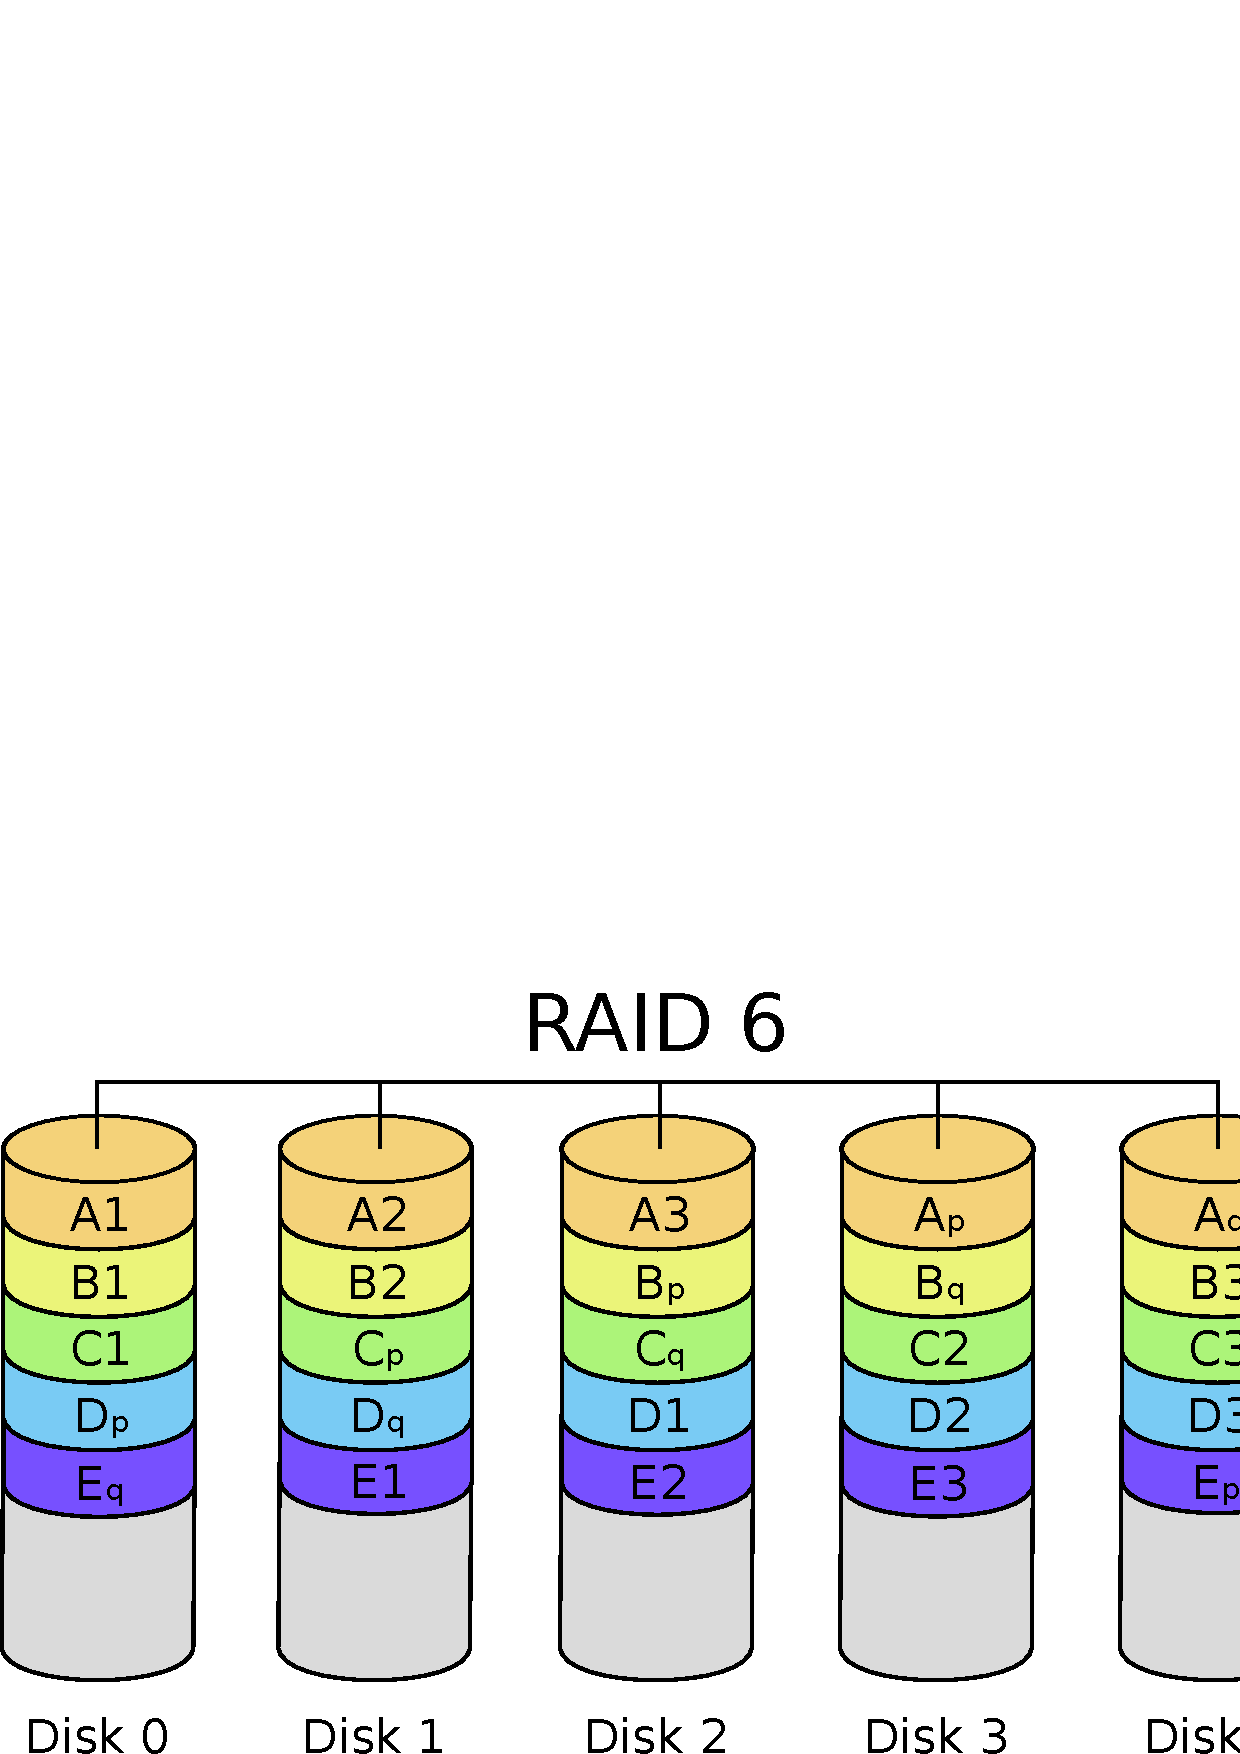
\includegraphics[width=\textwidth]{raid6.pdf} \\
	Definition: p and q are called syndromes.
\end{frame}

\section{Parity}
\subsection*{}
\begin{frame}
	Calculation of two syndromes:
	\begin{itemize}
		\item P: XOR all stripes (like in RAID 5)
		\item Q: XOR shifted  versions of the stripes
	\end{itemize}
\end{frame}

\begin{frame}
	\frametitle{Formulas (For the sake of completeness)}
	\begin{eqnarray}
		P &=& D_0 \oplus D_1 \oplus D_2 \oplus \dotsc \oplus D_n \\
		Q &=& g^0D_0 \oplus g^1D_1 \oplus g^2D_2 \oplus \dotsc g^nD_n 
	\end{eqnarray}
	where g is a generator of a Galois Field. 
\end{frame}

\section{Questions?}
\subsection*{}

\begin{frame}
	\frametitle{Questions?}
	\begin{center}
		\large Questions?
	\end{center}
\end{frame}

\end{document}
